Considere una función de producción Cobb-Douglas \[ Q = \alpha_{0}\prod_{m=1}^{M} x^{\alpha}_{m}. \] La maximización de ganancias con un precio de producción determinado de manera exógena exige que la empresa maximice la producción para un nivel de costo dado $C$ (o minimizar los costos para una producción dada $Q$). El lagrangeano para el problema de maximización es \[ \Lambda=\alpha_{0}\prod x^{\alpha_{m}}_{m} + \lambda(C-\bm{p}^{\prime}\bm{x}), \] donde $\bm{p}$ es el vector de los precios del factor $M$. Las condiciones necesarias para maximizar esta función son \[ \frac{\partial\Lambda}{\partial x_{m}}=\frac{\alpha_{m}Q}{x_{m}}-\lambda p_{m}=0\text{ y }\frac{\partial\Lambda}{\partial\lambda}=C-p^{\prime}\bm{x}=0. \]
La solución conjunta proporciona $x_{m}\left(Q, \bm{p}\right) $ y $\lambda\left(Q, \bm{p}\right)$. El costo total de producción es \[ \sum_{m=1}^{M}p_{m}x_{m}=\sum_{m=1}^{M}\frac{\alpha_{m}Q}{\lambda}. \]
El costo compartido asignado al $m$--ésimo factor es \[ \frac{p_{m}x_{m}}{\sum_{m=1}^{M}p_{m}x_{m}}= \frac{\alpha_{m}}
{\sum_{m=1}^{M}\alpha_{m}}=\beta_{m}. \]
El modelo completo es\footnote{Dejamos esto como ejercicio}
\begin{align*}\label{eq:mpdel}
\ln(C)&=\beta_{0} + \beta_{q} \ln Q + \sum_{m=1}^{M}\beta_{m} \ln p_{m} + \varepsilon_{c}\\
s_{m}&=\beta_{m}+\varepsilon_{m},\quad m=1,\ldots,M.
\end{align*}
% TODO: Refereenciar 6.17
Algebraicamente, $\sum_{m=1}^{M}\beta_{m}=1$ y $\sum_{m=1}^{M}s_{m} = 1$. (Este es el análisis de función de costo iniciado en el ejemplo 6.17. Regresaremos a esa aplicación a continuación.) Los costos compartidos también sumarán idénticamente a uno en los datos. Por lo tanto, se deduce que $\sum_{m=1}^{M}\varepsilon_{m}=0$ en cada dato punto por lo que el sistema es singular. Por el momento, ignore la función de costo. Deje que la $M\times1$ el vector de perturbación de las acciones será $\bm{\varepsilon}={\left[\varepsilon_{1}, \varepsilon_{2},\cdots,\varepsilon_{m}\right]}^{\prime}$. Porque $\bm{\varepsilon}^{\prime}\bm{i}=0$, donde $\bm{i}$ es una columna de 1s, se deduce que $E[\bm{\varepsilon}\bm{\varepsilon}^{\prime}\bm{i}]=\bm{\sum}\bm{i}=0$, lo que implica que $\bm{\sum}$ es singular.

Por lo tanto, los métodos de las secciones anteriores no se pueden usar aquí. (Debes verificar que la matriz de covarianza de \emph{muestra} de los residuos de $OLS$ también será singular).

La solución al problema de la singularidad parece ser soltar una de las ecuaciones, estimar el residuo y resolver el último parámetro del otro $M-1$. La restricción $\sum_{m=1}^{M}\beta_{m}=1$ establece que la función de costo debe ser homogénea de grado uno en los precios. Si imponemos la restricción
\begin{equation}\label{eq:betaestimaters}
\beta_{M} = 1 - \beta_{1} -\beta_{2} - \cdots - \beta_{M-1},
\end{equation}

entonces el sistema se reduce a uno no singular,
\begin{align*}
\ln\left(\frac{C}{p_{m}}\right)
&=\beta_{0}+\beta_{q}\ln Q + \sum_{m=1}^{M-1}\beta_{m}\ln\left(\frac{p_{m}}{p_{M}}\right)+\varepsilon_{c},\\
s_{m}
&=\beta_{m} + \epsilon_{m},\quad m=1,\ldots, M-1.
\end{align*}

Este sistema proporciona estimaciones de $\beta_{0}, \beta_{q}$ y $\beta_{1},\ldots,\beta_{M- 1}$. El último parámetro es estimado usando~\eqref{eq:betaestimaters}. Es irrelevante qué factor se elige como numerario; FGLS será \textbf{invariante} a qué factor se elige.

\begin{example}[Función de costo de Cobb-Douglas]
El estudio de Nerlove (1963) sobre la industria de la energía eléctrica que examinamos en el ejemplo 6.6 proporciona una aplicación del modelo de función de costo Cobb-Douglas. Sus estimados de mínimos cuadrados ordinarios de los parámetros se enumeraron en el ejemplo 6.6. Entre los resultados hay (desafortunadamente) un negativo coeficiente de capital en tres de las seis regresiones. Nerlove también encontró que el simple modelo de Cobb-Douglas no era una cuenta adecuada para la relación entre el producto y el costo promedio. Christensen y Greene (1976) analizaron más a fondo los datos de Nerlove y argumentaron que el conjunto de datos con los datos de costos compartidos para estimar el \textbf{sistema de demanda completo}. Cuadro del apéndice F6.2 enumera las 145 observaciones de Nerlove con los datos de costos compartidos de Christensen y Greene. El costo es el costo total de generación en millones de dólares, la producción es en millones de kilovatios-hora, el precio del capital es un índice de costos de construcción, la tasa salarial es en dólares por hora para producción y mantenimiento, el precio del combustible es un índice del costo por BTU del combustible comprado por las empresas, y los datos reflejan los costos de producción de 1955. Las estimaciones de regresión se dan en la Tabla 10.4.

Los estimados de mínimos cuadrados de la función de costo Cobb-Douglas se dan en la primera columna. El coeficiente sobre el capital es negativo. Porque $\beta_{m}=\beta_{q}\partial\ln Q/0\ln x_{m}$, es decir, un positivo múltiplo de la elasticidad de salida del factor $i$--ésimo; este hallazgo es preocupante. La tercera columna presenta las restricciones de las estimaciones FGLS. Para obtener el estimador restringido, fijamos el modelo en forma del estimador SUR agrupado en (10-20),
\end{example}
\[ \bm{y}=
\begin{bmatrix}
\bm{\ln(C/P_{f})} \\
\bm{s_{k}} \\
\bm{s_{l}}
\end{bmatrix} = \begin{bmatrix}
\bm{i} & \bm{\ln(Q)} & \bm{\ln(P_{k} / P_{f})} & \bm{\ln(P_{l} / P_{f})}\\
\bm{0} & \bm{0} & \bm{i} & \bm{0} \\\
\bm{0} & \bm{0} & \bm{0} & \bm{i}
\end{bmatrix}\begin{pmatrix}
\beta_{0}\\
\beta_{q}\\
\beta_{k}\\
\beta_{l}
\end{pmatrix} + \begin{bmatrix}
\bm{\epsilon}_{c}\\
\bm{\epsilon}_{k}\\
\bm{\epsilon}_{l}
\end{bmatrix}.
\]
Note que esta formulación impone las restricciones $\beta_{1}=\alpha_{3}$ y $\gamma_{1}=\alpha_{4}$ en % TODO: 
Existen $3\left(145\right)=435$ observaciones en las matrices de datos. %TODO: El estimador es entonces FGLS, como es mostrado en
Las estimaciones de la economía de escala en el modelo de Cobb-Douglas son $\frac{1}{\beta_{q}}=1.39$ (primera columna) y (tercera columna), el cual sugiere algún incremento de retorno a escala. Nerlove, sin embargo, encontró evidencia que en tamaños de empresas extremadamente grandes, las economías a escalas disminuyeron y eventualmente desaparecieron. Para dar cuenta de esto (esencialmene una curva de costo promedio clásica en forma de $U$), él agregó un término cuadrático en la salida logarítmica en la función de costo. La única ecuación y los estimadores FGLS dieron en el segundo y cuarto conjunto de resultados.

La salida cuadrática da la función de costo promedio y la esperada forma de $U$. Podemos determinar el punto donde el costo promedio alcanza su mínimo al igualar $\partial\ln C/\partial\ln Q$ a $1$. Este es $Q^{\ast}=\exp\left[\left(1-\beta_{q}\right)/\left(2\beta_{qq}\right)\right]$. Usando los estimadores FGLS, su valor es $Q^{\ast}=4.669$. Alrededor del $85$\% de las empresas en la muestra obtuvieron menos que eso, así por estos estimadores, muchas empresas en la muestra aún no habían agotado las economías de escala disponible.
~\ref{tb:predicted}

Tenga en cuenta que esta formulación impone las restricciones $\beta_{1} = \alpha_{3}$ y $\gamma_{1} = \alpha_{4}$ en (10-4). Existen 3 (145) = 435 observaciones en las matrices de datos. El estimador es entonces FGLS, como se muestra en (10-22) Se agrega una columna adicional para el modelo de registro cuadrático. Dos cosas a tener en cuenta son las
errores estándar dramáticamente más pequeños y la estimación ahora positiva (y razonable) de la coeficiente de capital Las estimaciones de las economías de escala en el modelo básico de Cobb-Douglas son
$1/\beta_{q}=1.39$ (columna 1) y 1.31 (columna 3), lo que sugiere algunos rendimientos crecientes a escala.
Sin embargo, Nerlove había encontrado evidencia de que a tamaños de empresa extremadamente grandes, economías de escala
disminuyó y finalmente desapareció. Para dar cuenta de esto (esencialmente un clásico en forma de U-curva de costo promedio), agregó un término cuadrático en la producción de registro en la función de costo. los La ecuación única y las estimaciones de FGLS se dan en el segundo y cuarto conjuntos de resultados.
El término de salida cuadrática le da a la función de costo promedio la forma de U esperada. Nosotros puede determinar el punto donde el costo promedio alcanza su mínimo al igualar $d\ln C/d\ln Q$ a 1. Esto es $Q^{\ast}=\exp\left[(1-\beta_{q})/(2\beta_{qq})\right]$. Usando las estimaciones de $FGLS$, este valor es $Q^{\ast}=4,669$.
(La aplicación 5 considera usar el método delta para construir un intervalo de confianza para $Q^{\ast}$).
Alrededor de $85$ de las empresas de la muestra tuvieron una producción inferior a esta, por lo que según estas estimaciones, la mayoría de las empresas de la muestra aún no habían agotado las economías de escala disponibles. La figura~\ref{fg:predicted} muestra costos promedio predichos y reales para la muestra. (Para obtener una escala razonable, la más pequeña
un tercio de las empresas se omiten de la figura.) Se calculan los costos promedio predichos en los promedios de muestra de los precios de entrada. La figura revela que eso más allá de un a pequeña escala, las economías de escala, aunque quizás estadísticamente significativas, son económicamente bastante pequeño.
\begin{table}[ht!]
	\begin{tabular}{lccccc}
		& & \textbf{Mínimos cuadrados ordinarios} & &\textbf{ Restricciones feasibles GLS} & \\
		\hline
		Constante	& $\beta_{0}$ & $-4.686$ & $-3.764$ & $-7.069$ & $-5.707$\\
			&  & $\left(0.885\right)$ & $\left(0.702\right)$ & $\left(0.107\right)$ & $\left(0.165\right)$\\
		$\ln$ Salida	& $\beta_{q}$ & $0.721$ & $0.153$ & $0.766$ & $0.239$\\
		&  & $\left(0.0174\right)$ & $\left(0.0618\right)$ & $\left(0.0154\right)$ & $\left(0.0587\right)$\\
		$\ln^{2}$ Salida & $\beta_{qq}$ &  &  $0.0505$ & & $0.0451$ \\
		 &  &  &  $\left(0.0054\right)$ & & $\left(0.00508\right)$ \\
		$\ln P_{\text{capital}}$	& $\beta_{k}$ & $-0.0085$ & $0.0739$ & $0.424$ & $0.425$ \\
		& & $\left(0.191\right)$ & $\left(0.150\right)$ & $\left(0.00946\right)$ & $\left(0.00943\right)$ \\
		$\ln P_{\text{trabajo}}$	& $\beta_{l}$ & $0.594$& $0.481$ & $0.106$ & $0.106$\\
		& & $\left(0.205\right)$ & $\left(0.161\right)$ & $\left(0.00386\right)$ & $\left(0.00380\right)$\\
		$\ln P_{\text{combustible}}$	& $\beta_{f}$ & $0.414$ & $0.445$ & $0.470$ & $0.470$\\
		&  & $\left(0.0989\right)$ & $\left(0.0777\right)$ & $\left(0.0101\right)$ & $\left(0.0100\right)$\\
		\hline
	\end{tabular}
	\caption{Estimados de la función de costos (Errores estimados estándar en paréntesis).}
\end{table}

\begin{figure}
	\centering
	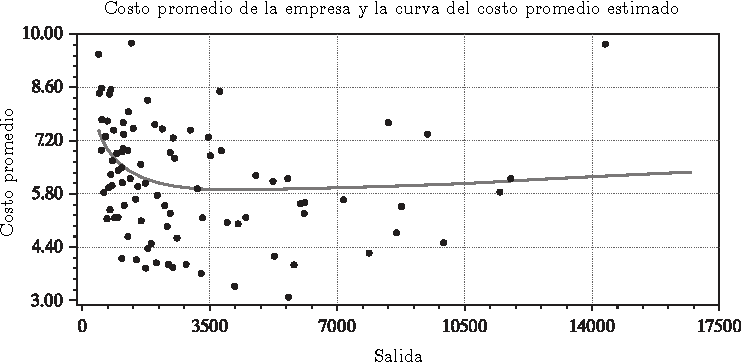
\includegraphics[width=0.6\paperwidth]{predictedaverage}
	\caption{Gráfica del costo promedio predecido.}\label{fg:predicted}
\end{figure}